\chapter{Application Window} \label{ch: application-window}

\begin{figure}[H]
	\centering
	\includesvg[scale=1]{images//app_window}
	\caption{Application Window.}
\end{figure}


The application window is the main container that holds all interface elements and the backend. It provides users with a cohesive environment to configure, run, and analyze the array with various parameters.

\section{\acf{gui}}

\begin{figure}[H]
	\centering
	\includesvg[scale=1]{images//window}
	\caption{Foundational \ac{gui} idea for the application window.}
\end{figure}

The \ac{gui} will consists of primarily two panes. Pane-1 will be for the user to input their configurations and settings. And Pane-2 will be for the visualizing the desired plot based on the user-defined settings. Typical parameters available will be,

\begin{itemize}
	\item Frequency
	\item inter-element spacing
	\item number elements
	\item array configurations
	\item angle-of arrival
\end{itemize}

\section{Signal Processing Backend}

This serves as the core engine that connects the user interface with the signal processing library. It receives configuration parameters from the GUI and uses them to initialize or update the processing chain. This backend handles tasks like generating steering vectors, applying beamforming algorithms, and performing DoA estimation using synthetic data. It communicates with the processing library and returns the computed results, which then can be plotted using the plotting library. This architecture ensures a modular responsive, and extensible system.

\section{Flow Graph Generator}

The Flow Graph Generator is a key component that automatically builds and configures a signal processing flow based on user input in \acl{gr}. Its main purpose is to translate high-level user-defined parameters into a structured and executable \ac{gr} flowgraph. This generator acts as a bridge between user-friendly GUI controls and the underlying processing blocks, ensuring that the right sequence of blocks is instantiated and connected in the \acf{grc}.

\section{Plotting library}

The Plotting Library is responsible for rendering all visual outputs in the application. It receives numerical data—like spatial spectra, array responses, or estimated angles—from the signal processing backend and generates clear, interactive plots in the Visualization Window (Pane-2). It includes different plotting methods like,

\begin{itemize}
	\item Contour plot
	\item Polar plot
	\item Cartesian plot
\end{itemize}

\clearpage
\begin{figure}[H]
	\centering
	\hspace*{-1.8cm}
	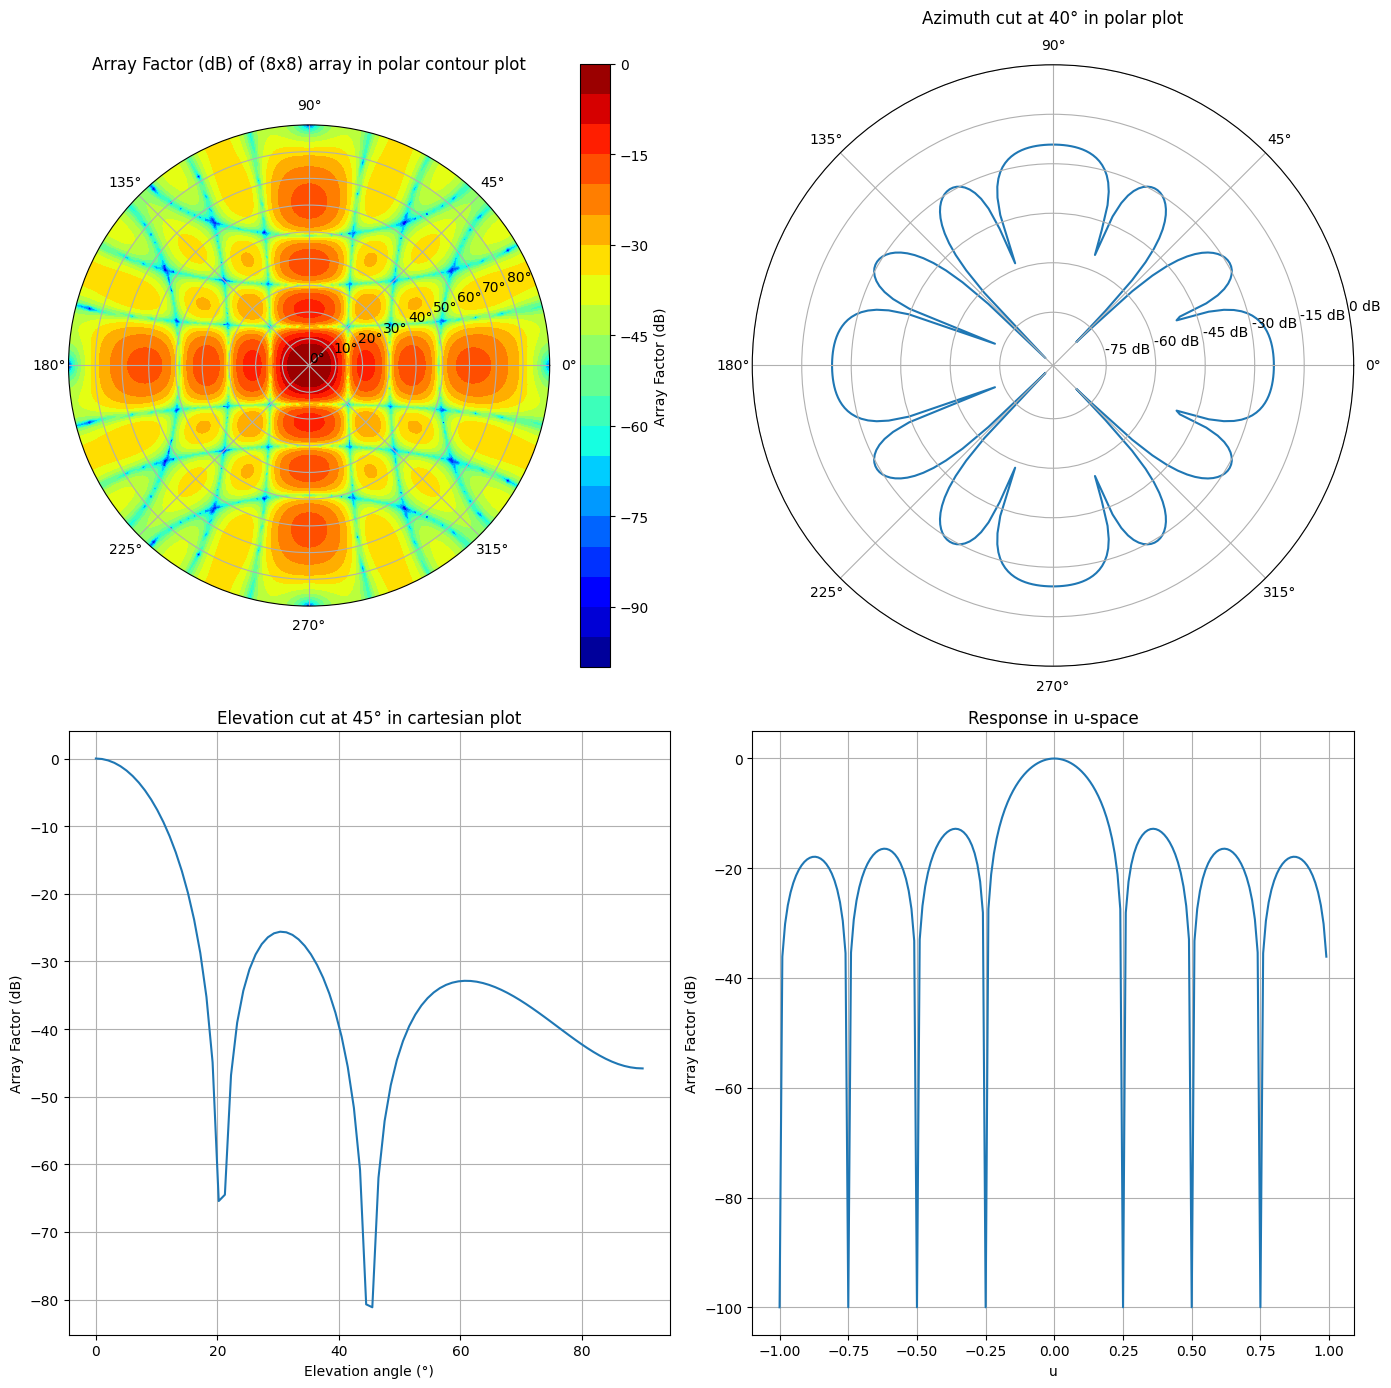
\includegraphics[scale=0.56]{images//plots}
	\caption{Different pattern visualization of an 8$\times$8 array.}
\end{figure}